% =============================================================================================
%  Choisir les nouveaux calculs quand l'objectif est la vitesse VPP : comment le plan séquentiel
%  de Le Gratiet & Cannamela a été adapté. Note pédagogique (5 pages).
%  Figure et valeurs : ..\..\.venv-mds\Scripts\python scripts\fig_selection.py
%  Compilation       : tectonic -X compile selection_points_vpp.tex --outdir build
% =============================================================================================
\documentclass[11pt,a4paper]{article}
\usepackage{fontspec}
\usepackage[french]{babel}
\usepackage{csquotes}
\usepackage[a4paper,margin=2.0cm,top=1.6cm,bottom=1.8cm]{geometry}
\usepackage{microtype}
\usepackage{amsmath,amssymb,mathtools,bm}
\usepackage{xcolor}
\usepackage{graphicx}
\usepackage{booktabs,tabularx,array}
\usepackage{enumitem}
\usepackage{caption}
\usepackage[most]{tcolorbox}
\usepackage{titlesec}
\usepackage[hidelinks,unicode]{hyperref}

\hypersetup{colorlinks=true,linkcolor=blue!50!black,citecolor=green!40!black,
            urlcolor=blue!60!black,pdftitle={Choisir les nouveaux calculs pour la VPP}}
\setlength{\parindent}{0pt}
\setlength{\parskip}{0.4em}
\setlist{itemsep=0.1em,topsep=0.2em,leftmargin=1.3em}
\renewcommand{\arraystretch}{1.12}
\titleformat{\section}{\normalfont\large\bfseries\color{blue!40!black}}{\thesection}{0.6em}{}
\titlespacing*{\section}{0pt}{0.8em}{0.25em}
\captionsetup{font=small,labelfont=bf,margin=0.3cm}

% encadrés du document Doc-GP-mfego (preambule.tex)
\tcbset{enhanced,breakable,boxrule=0.6pt,arc=1.5mm,left=2mm,right=2mm,top=0.8mm,bottom=0.8mm,
        fonttitle=\bfseries\small\hypersetup{citecolor=yellow!60!white,linkcolor=yellow!60!white},
        before skip=0.6em,after skip=0.6em}
\newtcolorbox{theorie}[1][]{colback=blue!3,colframe=blue!45!black,
  title={Théorie\ifx&#1&\else~— #1\fi}}
\newtcolorbox{refbox}[1][]{colback=gray!5,colframe=gray!55!black,
  title={Ce que disent les références\ifx&#1&\else~— #1\fi}}
\newtcolorbox{danslecode}[1][]{colback=green!3,colframe=green!35!black,
  title={Dans le code\ifx&#1&\else~— #1\fi}}
\newtcolorbox{subtilite}[1][]{colback=orange!4,colframe=orange!70!black,
  title={Subtilité\ifx&#1&\else~— #1\fi}}
\newtcolorbox{aretenir}[1][]{colback=violet!4,colframe=violet!60!black,
  title={À retenir\ifx&#1&\else~— #1\fi}}

\newcommand{\vx}{\bm{x}}
\newcommand{\vz}{\bm{z}}
\newcommand{\va}{\bm{a}}
\newcommand{\vc}{\bm{c}}
\newcommand{\tp}{^{\mathsf{T}}}
\newcommand{\py}[1]{\texttt{#1}}
\DeclareMathOperator{\Var}{Var}
\DeclareMathOperator{\Cov}{Cov}
\DeclareMathOperator*{\argmax}{arg\,max}

% Generated by scripts/fig_selection.py: do not edit by hand
\newcommand{\valRhoExemple}{0{,}94}
\newcommand{\valXGlobal}{0{,}33}
\newcommand{\valNiveauGlobal}{2}
\newcommand{\valXCible}{0{,}83}
\newcommand{\valNiveauCible}{2}
\newcommand{\valPartGlobal}{9}
\newcommand{\valReductionCible}{81}
\newcommand{\valRendementAvantA}{0{,}36}
\newcommand{\valRendementAvantB}{0{,}17}
\newcommand{\valRendementAvantC}{0{,}02}
\newcommand{\valRendementAvantD}{0{,}00}
\newcommand{\valLot}{0{,}83\,(HF), 0{,}90\,(BF), 0{,}90\,(HF), 0{,}88\,(BF)}
\newcommand{\valVitesseEtat}{18{,}57}
\newcommand{\valTableSensibilites}{$F_x$ & -0{,}0130 & 111{,}0 & 0{,}36 & 0{,}276 & 3{,}97 & 95{,}4 \\
$F_y$ & -0{,}3145 & -0{,}5 & 0{,}87 & 0{,}028 & 0{,}04 & 0{,}0 \\
$F_z$ & 0{,}2186 & 6{,}9 & 0{,}67 & 0{,}030 & 0{,}46 & 1{,}3 \\
$M_x$ & -0{,}5713 & 4{,}8 & 1{,}54 & 0{,}027 & 0{,}74 & 3{,}3 \\
$M_y$ & 0{,}0819 & 0{,}6 & 0{,}62 & 0{,}076 & 0{,}04 & 0{,}0 \\
$M_z$ & 0{,}0770 & 0{,}0 & 0{,}38 & 0{,}050 & 0{,}00 & 0{,}0 \\}
\newcommand{\valSigmaVitesse}{4{,}1}


\begin{document}

{\centering
{\Large\bfseries\color{blue!40!black} Choisir les nouveaux calculs quand l'objectif est la vitesse VPP\par}
\vspace{0.15em}
{\large Comment le plan séquentiel de Le Gratiet \& Cannamela a été adapté au cas du C-foil\par}
\vspace{0.2em}
{\small Note pédagogique · \py{vpp\_acceleration} · 23/10/2026\par}}

\vspace{0.4em}
\textbf{Ce que cette note explique.} À chaque pas, l'algorithme doit répondre à deux questions : \emph{où}
lancer un calcul de code, et \emph{à quel niveau} (BF : NPLLT × NeuralFoil, ou HF : NPLLT × XFOIL). On
part de la stratégie de Le Gratiet \& Cannamela~\cite{LGC15}, que tu connais. On montre ce qu'il a fallu
changer parce que la question n'est plus \enquote{un bon modèle partout}, mais \enquote{la bonne vitesse là où
la VPP travaille}, et l'on écrit \textbf{chaque hypothèse} faite en chemin (récapitulées au §\,7). Le modèle
lui-même est le co-krigeage AR(1) imbriqué du document mfego (chapitres 5 et 6), utilisé tel quel, une fois
par coefficient du torseur.

% ---------------------------------------------------------------------------------------------
\section{Le point de départ : la stratégie de Le Gratiet \& Cannamela}
% ---------------------------------------------------------------------------------------------
\begin{refbox}[\cite{LGC15}, §3 et algorithme 1]
Le but est un modèle du niveau haut $Z_2$ précis \textbf{sur tout le domaine} $Q$. L'erreur visée est
l'IMSE, $\int_Q \Var[Z_2(\vx)\mid\text{données}]\,d\vx$. Chaque pas se fait en deux temps :
\begin{enumerate}
  \item \textbf{Où :} au maximum d'une variance de prédiction \enquote{ajustée} par validation croisée
        (leave-one-out), dans la cellule de Voronoï des points existants ;
  \item \textbf{Jusqu'à quel niveau :} en comparant, pour ce point, la réduction d'IMSE de chaque niveau
        rapportée au rapport des coûts. Calculer au niveau 2 impose de calculer aussi le niveau 1 : le plan
        reste imbriqué.
\end{enumerate}
\end{refbox}

L'idée de fond, que nous gardons, est celle des stratégies de réduction d'incertitude (SUR~\cite{Bect12}) :
\textbf{on sait, avant de lancer un calcul, combien il réduira la variance du modèle}. La variance d'un GP ne
dépend que des positions des observations, et non des valeurs que le code rendra.

\begin{theorie}[le gain exact d'un calcul]
Ajouter le point $\vx_m$ au niveau $l$, c'est observer $\vx_m$ à tous les niveaux $j\le l$ qui y manquent.
Notons :
\begin{itemize}
  \item $\vc(\vx)$ : la covariance a posteriori entre $Z_2(\vx)$ et ces nouvelles observations ;
  \item $S$ : la covariance a posteriori de ces observations, bruit compris.
\end{itemize}
La variance de $Z_2(\vx)$ baisse alors exactement de $\vc(\vx)\tp S^{-1}\vc(\vx)$. Le gain intégré est
\begin{equation}\label{eq:gain}
  G(\vx_m,l)=\int \vc(\vx)\tp S^{-1}\vc(\vx)\;\mu(d\vx)\;\approx\;\frac1N\sum_{i=1}^{N}\vc(\vx_i)\tp S^{-1}\vc(\vx_i),
\end{equation}
où $\mu$ est la \emph{mesure d'intégration} : uniforme sur $Q$ chez \cite{LGC15}, et $\{\vx_i\}$ des points
qui l'échantillonnent. C'est le critère ALC (\enquote{active learning Cohn}~\cite{Cohn96}). La formule est
exacte, à hyperparamètres fixés, avec la covariance jointe des deux niveaux.
\end{theorie}

\textbf{Ce que nous avions déjà changé avant la VPP} (note du 19/10, études du 21/10) :
\begin{itemize}
  \item \textbf{Un choix conjoint du point et du niveau}, au meilleur rendement $G(\vx_m,l)/C(\vx_m,l)$ parmi
        tous les couples, au lieu du point au maximum de variance puis du niveau. Le maximum de variance
        attirait les points sur les bords et privait la HF de points (Hartmann 6D). Le choix conjoint ALC
        corrige cela : erreur de 0,69 à 0,71, contre 0,82 pour un LHS.
  \item \textbf{Le gain de chaque niveau mesuré sur la sortie HF.} La règle publiée compare une réduction BF à
        une réduction HF, et il lui manque un facteur $\rho^2$.
  \item \textbf{Ni ajustement par validation croisée} (nos sorties sont lisses), \textbf{ni $\rho$ libre} :
        un prior $\mathcal{N}(1,2^2)$ le borne (la version \enquote{v2}). Sans ce prior, $\rho$ montait
        jusqu'à 30.
\end{itemize}

% ---------------------------------------------------------------------------------------------
\section{Ce que la VPP change dans la question}
% ---------------------------------------------------------------------------------------------
Nous ne voulons pas un torseur juste \emph{partout} : nous voulons savoir \textbf{quelle section fait aller
le bateau le plus vite}. Trois différences en découlent.
\begin{enumerate}
  \item \textbf{La grandeur d'intérêt est la vitesse $V$}, et non les 7 coefficients. Une erreur sur la
        traînée et une erreur de même taille sur un moment n'ont pas le même effet sur $V$.
  \item \textbf{La VPP n'interroge le foil qu'autour de l'équilibre.} Pour une section donnée, à chaque
        condition de vent, la VPP cherche une attitude d'équilibre $\va=(\text{cant},\text{rake},\text{yaw})$.
        Elle n'évalue le foil qu'au voisinage de cette attitude. Le reste du domaine (13 dimensions : 10
        scores de section et 3 angles) lui est inutile.
  \item \textbf{Les sections qui comptent changent pendant la recherche.} Ce sont le titulaire (la meilleure
        section du moment) et ses concurrentes.
\end{enumerate}
Chaque différence donne une adaptation du critère~\eqref{eq:gain}, présentée dans les trois sections suivantes.

% ---------------------------------------------------------------------------------------------
\section{Première adaptation : pondérer les sorties par leur effet sur la vitesse}
% ---------------------------------------------------------------------------------------------
\begin{theorie}[de l'erreur sur le torseur à l'erreur sur la vitesse]
À un état d'équilibre, une petite erreur $\delta C_k$ sur le coefficient $k$ change la vitesse
d'équilibre de $d_k\,\delta C_k$ environ, où $d_k=\partial V/\partial C_k$ (\textbf{hypothèse H4} :
premier ordre). Les 7 co-krigeages sont indépendants (\textbf{H5}). La variance de la vitesse prédite est
donc
\begin{equation}\label{eq:varV}
  \Var V \;\approx\; \sum_{k=1}^{6} d_k^2\,s_k^2(\vx),
\end{equation}
avec $s_k^2$ la variance a posteriori du co-krigeage $k$. Cpmin n'agit pas sur la vitesse : son poids est
nul.
\end{theorie}

\textbf{Pourquoi c'est indispensable.} Voici les vrais chiffres du 3\textsuperscript{e} run, à la meilleure
section, condition 45°/16 nd (vitesse \valVitesseEtat{} nd) :

\begin{center}\small
\begin{tabular}{@{}lrrrrrr@{}}
\toprule
 & $\mu_k$ & $d_k$ [nd/unité] & $s_k$ [$10^{-4}$] & $s_k/|\mu_k|$ [\%] & $|d_k|\,s_k$ [$10^{-3}$ nd] & part de $\Var V$ [\%] \\
\midrule
\valTableSensibilites
\bottomrule
\end{tabular}
\end{center}

\begin{itemize}
  \item \textbf{La traînée $F_x$ fait 95 \% de l'incertitude de vitesse.} Ce n'est pourtant pas le
        coefficient le plus incertain en valeur absolue : $M_x$ et $F_y$ le sont davantage.
  \item \textbf{La raison est physique.} Si le surrogate surestime un peu l'effort latéral $F_y$, la VPP
        retrouve l'équilibre avec une dérive à peine différente, et la vitesse ne bouge presque pas
        ($d_{F_y}\approx-0{,}5$). Une erreur de traînée, elle, se paie directement en vitesse
        ($d_{F_x}\approx111$ : 1 \% d'erreur sur $F_x$ vaut environ 0,014 nd).
  \item \textbf{La conséquence.} Un critère non pondéré aurait dépensé des calculs à apprendre $M_x$. Le
        critère pondéré les dépense sur la traînée.
\end{itemize}

\begin{danslecode}
\begin{itemize}
  \item Les $d_{kc}$ (coefficient $k$, condition $c$) sont calculés par \textbf{différences finies avec la
        VPP complète}, au titulaire : on décale la sortie $k$ du surrogate d'environ 3 \% et l'on refait le
        solve. Cela fait 6 solves décalés par condition, chacun avec son solve de base dans le même
        processus, refaits une mise à jour sur trois.
  \item Le poids d'une sortie est la moyenne sur les conditions, $w_k=\frac15\sum_c d_{kc}^2$ (\textbf{H6}).
  \item Le critère~\eqref{eq:gain} devient $\sum_{k\le6} w_k\,G_k(\vx_m,l)$, une somme des gains des 6
        co-krigeages.
\end{itemize}
\end{danslecode}

\begin{subtilite}[ce que ces hypothèses négligent]
\begin{itemize}
  \item \textbf{H5} ignore que les erreurs de $F_y$ et de $M_x$ sont liées physiquement : un même défaut de
        portance les produit toutes les deux.
  \item \textbf{H6} donne le même poids à toutes les conditions, alors que $d_{F_x}$ va de 84 (45°/12 nd) à
        302 (90°/14 nd). Un poids par état serait plus juste, et ne coûterait qu'une ligne : la moyenne de
        l'éq.~\eqref{eq:gain} deviendrait une moyenne pondérée.
  \item \textbf{H4} vaut tant que les erreurs restent petites devant ce qui déplace l'équilibre.
\end{itemize}
\end{subtilite}

% ---------------------------------------------------------------------------------------------
\section{Deuxième adaptation : intégrer là où la VPP travaille}
% ---------------------------------------------------------------------------------------------
Dans~\eqref{eq:gain}, seule la mesure $\mu$ change : au lieu du domaine entier, on intègre \textbf{autour des
états d'équilibre} des sections en compétition (\textbf{H7}).
\begin{itemize}
  \item \textbf{Les états :} à chaque mise à jour, 4 sections (le titulaire et ses 3 meilleures
        concurrentes) aux 5 conditions, soit 20 états.
  \item \textbf{Les nuages :} 16 points autour de chaque état, à section fixe, l'attitude variant de $\pm1°$
        en cant, $\pm0{,}3°$ en rake et $\pm1°$ en yaw. Un nuage plutôt que l'état seul, parce que l'équilibre
        se déplace quand le surrogate change : entre deux sections proches, de quelques dixièmes de degré.
\end{itemize}

\begin{figure}[h]
\centering
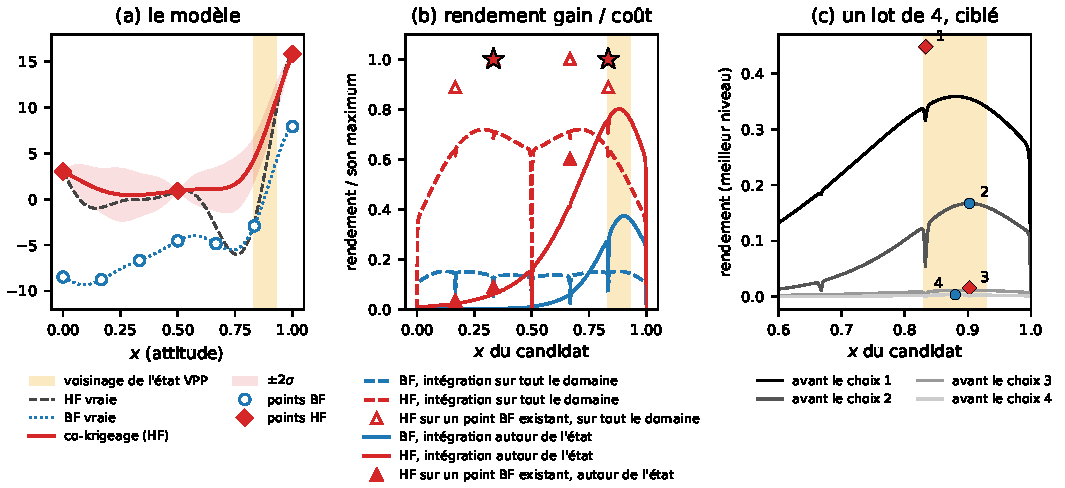
\includegraphics[width=\textwidth]{figures/fig_selection.pdf}
\caption{Exemple 1D à deux niveaux, calculé avec le code du dépôt : Forrester, BF à 7 points, HF à 3 points
imbriqués, $\hat\rho=\valRhoExemple$, coûts 1 et 2. La bande jaune est le voisinage d'un \enquote{état VPP}.
\textbf{(a)} Le co-krigeage HF et ses $\pm2\sigma$.
\textbf{(b)} Le rendement de chaque candidat et niveau : intégration sur tout le domaine (pointillés, la
cible de \cite{LGC15}) ou autour de l'état (traits pleins). Les étoiles marquent les deux choix.
\textbf{(c)} Le rendement ciblé avant chacun des 4 choix d'un lot (§\,6) : losanges HF, ronds BF.}
\label{fig:selection}
\end{figure}

\textbf{Ce que montre la figure~\ref{fig:selection}.}
\begin{itemize}
  \item \textbf{Le critère global} choisit un calcul HF en $x=\valXGlobal$, là où le modèle est le plus
        incertain \emph{en moyenne}.
  \item \textbf{Le critère ciblé} choisit un calcul HF en $x=\valXCible$, sur un point BF déjà calculé : la
        HF n'y coûte que 2.
  \item \textbf{Mesuré au voisinage de l'état,} le choix global ne retire que \valPartGlobal{}~\% de la
        variance que retire le choix ciblé. Le choix ciblé, à lui seul, retire \valReductionCible{}~\% de la
        variance locale.
\end{itemize}
C'est exactement l'effet recherché : chaque calcul sert la décision de la VPP. Sur un test de région (profil
4D, 20 graines), cette intégration ciblée a réduit l'erreur dans la région de 27 \% par rapport à un LHS
imbriqué.

\begin{theorie}[comment les nuages suivent la recherche]
Ce n'est plus de la planification d'expériences pure : le critère est couplé à l'optimiseur. À chaque mise à
jour :
\begin{enumerate}
  \item on crible 256 sections nouvelles avec le surrogate. Pour chacune, on calcule le gain de vitesse
        attendu, au premier ordre, plus $\kappa\,\sigma$ ($\kappa=1$, un optimisme face à l'incertitude, comme
        le critère UCB~\cite{Srinivas10}) ;
  \item les 3 meilleures passent à la VPP complète, avec le titulaire ;
  \item \textbf{leurs états deviennent les nouveaux points d'intégration.}
\end{enumerate}
Une section mal connue mais prometteuse entre donc dans le trio, attire des calculs, puis gagne ou est
écartée. C'est le mécanisme d'exploration. Le reste du domaine n'est raffiné que par corrélation : sa
précision globale n'est pas recherchée (le revers de H7).
\end{theorie}

% ---------------------------------------------------------------------------------------------
\section{Troisième adaptation : le choix du point, du niveau et le coût}
% ---------------------------------------------------------------------------------------------
Le choix final est un maximum de rendement sur un ensemble \emph{fini} de candidats (\textbf{H10}) :
\begin{equation}\label{eq:choix}
  (\vx^\star,l^\star)=\argmax_{m,\;l}\;\frac{\sum_{k\le6} w_k\,G_k(\vx_m,l)}{C(\vx_m,l)},\qquad
  C(\vx_m,l)=\sum_{j\le l,\ j\ \text{manquant en}\ \vx_m} c_j .
\end{equation}

\textbf{Les candidats} sont de trois sortes :
\begin{itemize}
  \item 500 points des nuages (autour des états) ;
  \item 256 points de tout le domaine, pour que le critère puisse aller ailleurs si c'est rentable ;
  \item les points BF qui n'ont pas encore de HF (au plus 512), où seule la HF est possible.
\end{itemize}

\textbf{Le coût cumulé} vient de l'imbrication (\textbf{H2}). Un point nouveau au niveau 2 coûte $c_1+c_2=3$,
une HF sur un point BF existant coûte $c_2=2$. La figure~1 le montre : le critère ciblé préfère une HF sur un
point BF voisin de l'état plutôt qu'un point neuf.

\textbf{Le rapport des coûts} est de 1 : 2 (\textbf{H8}). C'est celui du temps réel par choix, et non celui
des temps de calcul des codes. Les calculs d'un lot tournent en parallèle, et un choix coûte surtout le
temps de sélection, à peu près le même aux deux niveaux. Une HF n'allonge le lot que si sa section est
nouvelle (la polaire XFOIL, de 2 à 13 s). Au 2\textsuperscript{e} run, en séquentiel avec AVL en HF, le
rapport valait 1 : 6.

% ---------------------------------------------------------------------------------------------
\section{Seize calculs à la fois : le \enquote{kriging believer}}
% ---------------------------------------------------------------------------------------------
On ne prend pas simplement les 16 meilleurs rendements de~\eqref{eq:choix} : ce seraient 16 voisins du même
maximum, presque redondants. On choisit plutôt l'un après l'autre. Après chaque choix, on conditionne le
co-krigeage sur le point choisi \emph{comme s'il avait été calculé}, avec pour valeur provisoire sa moyenne
prédite (Ginsbourger et al.~\cite{GLC10}).

\textbf{Pourquoi c'est exact pour notre critère.} Le gain~\eqref{eq:gain} ne dépend que de la variance
a posteriori. La formule $k_n(\bm a,\bm b)=k(\bm a,\bm b)-\bm k(\bm a,X)K^{-1}\bm k(X,\bm b)$ ne contient pas
les valeurs observées. Le choix suivant voit donc exactement la variance que les choix précédents vont
retirer. La valeur provisoire, elle, laisse les moyennes inchangées : elle ne sert qu'à faire tourner le code,
et elle est remplacée par la vraie valeur après le calcul.

\textbf{Sur la figure~1(c)}, le lot ciblé de 4 donne \valLot.
\begin{itemize}
  \item Après les deux premiers choix, le rendement au voisinage de l'état s'effondre, de
        \valRendementAvantA{} à \valRendementAvantC{} : il est appris.
  \item Le 3\textsuperscript{e} choix ajoute la HF au point BF que le 2\textsuperscript{e} vient de prendre,
        ce qui respecte l'imbrication.
  \item Dans le vrai problème, avec 20 états, les choix suivants iraient vers d'autres états.
\end{itemize}

\begin{subtilite}[ce qui reste fixe pendant un lot (H9)]
Les hyperparamètres (longueurs de corrélation, $\rho$) ne changent pas pendant le lot. Ils ne sont
réestimés que lorsque le plan a grossi de 25 \% ; entre deux réestimations, on conditionne seulement. Le
critère se fie donc à des longueurs de corrélation estimées sur un plan un peu plus petit. Le lot dépend
aussi des sensibilités $d_k$ et des états de la dernière mise à jour.
\end{subtilite}

% ---------------------------------------------------------------------------------------------
\section{Les hypothèses, en un tableau}
% ---------------------------------------------------------------------------------------------
{\small
\begin{tabularx}{\linewidth}{@{}l>{\raggedright\arraybackslash}X>{\raggedright\arraybackslash}X>{\raggedright\arraybackslash}X@{}}
\toprule
 & Hypothèse & Pourquoi & Ce qu'on risque \\
\midrule
H1 & AR(1) à $\rho$ constant, un co-krigeage indépendant par coefficient, même plan & le modèle de \cite{LG}, validé sur nos cas ; un calcul donne tout le torseur & une corrélation BF/HF qui varie dans le domaine \\
H2 & plan imbriqué : la HF seulement là où la BF existe & condition du co-krigeage récursif & aucun, sinon le coût cumulé \\
H3 & choix conjoint (point, niveau) par l'ALC exact, sans ajustement LOO & bat le maximum de variance sur Hartmann 6D & suppose des hyperparamètres bien estimés \\
H4 & vitesse linéarisée en $\delta C_k$ & rend le critère calculable & faux si les erreurs déplacent beaucoup l'équilibre \\
H5 & erreurs des 7 sorties indépendantes & 7 GP indépendants & corrélations physiques ignorées ($F_y$, $M_x$) \\
H6 & un poids par sortie, moyenne sur les conditions & simple & sous-pondère les conditions sensibles (90°/14) \\
H7 & intégration autour des états VPP de 4 sections & seule zone utile à la décision & le reste du domaine peu appris \\
H8 & coûts 1 : 2 en temps réel par choix & calculs parallèles & mal réglé, il gaspille les HF ou les BF \\
H9 & hyperparamètres et sensibilités figés pendant un lot & le gain doit être calculable sans relancer les codes & un lot de 16 un peu moins bien placé \\
H10 & maximum sur un ensemble fini de candidats & le calcul vectorisé du gain & un meilleur point entre les candidats \\
\bottomrule
\end{tabularx}}

% ---------------------------------------------------------------------------------------------
\section{Le cœur et les ajouts}
% ---------------------------------------------------------------------------------------------
Tu as raison : le code est devenu plus compliqué que ce que nous avions convenu. Pour le comprendre, il suffit
de garder le \textbf{cœur}, qui tient en quatre lignes :
\begin{enumerate}
  \item le co-krigeage AR(1) de \cite{LG}, un par coefficient (H1, H2) ;
  \item le gain exact~\eqref{eq:gain} et le choix au meilleur rendement~\eqref{eq:choix} (H3) ;
  \item la pondération par $(\partial V/\partial C_k)^2$ (H4–H6) ;
  \item l'intégration autour des états VPP, qui suivent la recherche (H7).
\end{enumerate}
Le reste sert à aller plus vite, et ne change pas la logique : les lots de 16 (§\,6), les processus
parallèles pour les codes et la VPP, les fils sur les 7 modèles, la prédiction \enquote{moyenne seule} pour la
VPP, la règle des 25 \% pour réestimer les hyperparamètres, et deux garde-fous (au plus 512 points BF sans HF
parmi les candidats, exclusion des points en échec). Avec un lot de 1 et sans processus parallèles, on
retrouve l'algorithme du 2\textsuperscript{e} run. Ces couches peuvent se ranger derrière une option, pour
que le cœur se lise d'un seul tenant.

\begin{thebibliography}{9}\footnotesize\setlength{\itemsep}{0pt}
\bibitem{LGC15} L. Le Gratiet, C. Cannamela, \emph{Cokriging-based sequential design strategies using fast
cross-validation techniques for multi-fidelity computer codes}, Technometrics 57(3), 418–427, 2015.
\bibitem{LG} L. Le Gratiet, \emph{Multi-fidelity Gaussian process regression for computer experiments},
thèse, Université Paris-Diderot, 2013.
\bibitem{Cohn96} D. Cohn, \emph{Neural network exploration using optimal experiment design}, Neural
Networks 9(6), 1996.
\bibitem{Bect12} J. Bect, D. Ginsbourger, L. Li, V. Picheny, E. Vazquez, \emph{Sequential design of computer
experiments for the estimation of a probability of failure}, Statistics and Computing 22, 2012.
\bibitem{GLC10} D. Ginsbourger, R. Le Riche, L. Carraro, \emph{Kriging is well-suited to parallelize
optimization}, in \emph{Computational Intelligence in Expensive Optimization Problems}, Springer, 2010.
\bibitem{Srinivas10} N. Srinivas, A. Krause, S. Kakade, M. Seeger, \emph{Gaussian process optimization in
the bandit setting: no regret and experimental design}, ICML 2010.
\end{thebibliography}

\end{document}
